\documentclass[12pt]{article}

\usepackage{xspace}
\usepackage{lineno}
\usepackage{setspace}
\usepackage{graphicx}
\usepackage{subfigure}
\usepackage{float}
\usepackage{color}
\usepackage{caption}
\usepackage[margin=1in]{geometry}
\usepackage{epstopdf}
\usepackage{natbib}
\usepackage{amsmath}

\begin{document}
\doublespacing
\linenumbers


\newcommand{\LLik}{\ensuremath{\text{\emph{L}}}\xspace}


\noindent RH: LANDERER ET AL.--- Estimating genetic load
% put in your own RH (running head)
% for POVs the RH is always POINT OF VIEW
\bigskip
\medskip
\begin{center}

% Insert your title:
\noindent{\Large \bf Estimating the genetic load of natural protein coding sequences using a phylogenetic framework.}
\bigskip


\noindent{C\textsc{EDRIC} ~{L\textsc{ANDERER}}$^{1,2,*}$,
B\textsc{RIAN} C.~ {O\textsc{MEARA}}$^{1,2}$,
\textsc{AND}
M\textsc{ICHAEL} A.~{G\textsc{ILCHRIST}}$^{1,2}$}

\end{center}

\vfill

{\small
\noindent$^{1}$Department of Ecology \& Evolutionary Biology, University of Tennessee, Knoxville, TN 37996-1610\\
\noindent$^{2}$National Institute for Mathematical and Biological Synthesis, Knoxville, TN 37996-3410\\
\noindent$^{*}$Corresponding author. E-mail:~cedric.landerer@gmail.com
}

\vfill
\centerline{Version dated: \today}
\vfill
\newpage



\begin{abstract}
Protein production is a very costly process every cell performs, resulting in selection for proteins that can perform their function most efficiently.
The efficacy of selection is limited by the effective population size $N_e$, leading to genetic load via the introduction of mutations.
As all proteins have to face this selection-mutation-drift barrier, we expect to find proteins near a fitness peak, but never at the peak.
Here, we assess the efficacy of selection on individual proteins and quantify the genetic load by phylogenetic inference of the optimal amino acid at each site using SelAC.
We compare our estimates of site specific amino acid fitness and genetic load to empirical estimates from deep mutation scanning experiments.
Our work demonstrates the shortcomings of empirical fitness estimates obtained under laboratory conditions and highlights the general applicability of SelAC.
Using model selection, we show that phylogenetic estimates of fitness are preferred over empirical estimates ($\Delta$AIC $ = 586$). 
Using the empirical estimates, the genotype with the highest fitness only shows $49\%$ sequence identity with the observed TEM variants.
Simulations reveal that the empirical fitness values do not adequately reflect natural evolution as we would not expect to observe the natural TEM sequence variants.
Furthermore, we demonstrate the generality of SelAC by estimating the genetic load of cytochrome B in whales.
These results indicate that genetic load varies greatly along cytochrome B.
\end{abstract}

\section*{Introduction}
\begin{itemize}
	\item NOTE: Use Substitutional Load instead (Kimura and Maruyama 1968)? Initial frequency implicit 1/2Ne?
	\item Genetic load is a measure of distance between the average genotype's fitness and the genotype with the highest fitness.
	\begin{itemize}
		\item The genotype with the highest fitness is assessed based on the set of observed genotypes.
		\item Mutation constantly introduces new, potentially deleterious mutations increasing the genetic load of a population.
		\item Genetic drift limits the efficacy of natural selection.
		\item Therefore, the optimal genotype is likely not among the observed genotypes.
		\item To remedy this, experimental procedures like deep mutation scanning can be employed to asses the fitness of genotypes.
	\end{itemize}
	\item Deep mutation scanning (DMS) requires a library of mutants for which the fitness should be assessed.
	\begin{itemize}
		\item This limits the application of DMS experiments to organisms that can be manipulated under laboratory conditions, and have a sufficiently short generation time.
		\item It also requires that artificial selection can be applied.
		\item This limits DMS experiments even further to proteins for which we can assume they respond to a singular stress factor.
		\item While it is save to ignore effects of mutation, the low population size does severely limit the efficacy of selection.
		\item It is therefore required to apply extremely strong selection pressure.
	\end{itemize}
	\item In this study, we assess how well DMS experiments are suited to assess genetic load produced by natural evolution.
	\begin{itemize}
		\item It has previously been demonstrated that incorporation of DMS experiments into phylogenetic approaches improve model fit when compared to classical approaches like GY94.
		\item However, model adequacy has not been assessed.
		\item First we show that the models fits achieved by the incorporation of DMS experiments can be improved upon using a novel phylogenetic framework, SelAC.
		\item We find that we would not expect to observe the natural TEM variants when simulating under the DMS inferred fitness landscape.
		\item We then compare the genetic load of natural TEM variants according to DMS and SelAC and show that DMS predicts an increased genetic load.
	\end{itemize}
	\item Having shown that SelAC provides more adequate inference of genetic load we further demonstrate its generality by assessing the genetic load of cytochrome B in whales, an organisms for which DMS experiments are not possible.
\end{itemize}

\section*{Results}
\begin{itemize}
	\item We used SelAC and phyDMS to compare model fits to TEM sequence variants.
	\begin{itemize}
		\item AIC values showed that SelAC provided an improved model fit (Tabel \ref{tab:AIC}).
		\item Ignoring the phylogenetic relationship, sequence comparison reveals that the sequence with the highest cumulative fitness according to DMS only shows $\sim49 \%$ agreement with the consensus of the observed TEM variants (Figure \ref{fig:sim_seqs_cons}).
		\item In contrast, the optimal amino acid sequence inferred by SelAC shows $99\%$ sequence similarity.
	\end{itemize}
	\item Simulations of sequence evolution using the site specific DMS fitness estimates show that DMS does not reflect natural sequence evolution.
	\begin{itemize}
		\item Assuming reasonable, but still small effective population sizes for \textit{E. coli} ($10,000 - 1,000,000$), we would expect to observe a sequence similarity of $\sim 70 \%$ (Figure \ref{fig:dms_sim}a).
		\item We also expect to only observed half the genetic load (Observed mean: $\sim 22$ v Expected mean: $\sim 10$) (Figure \ref{fig:gl_TEM_whale}a and \ref{fig:dms_sim}b)
		\item However, even with an effective population size as small as 100, we would expect a significantly lower genetic load than observed.
	\end{itemize}
	\item SelAC estimates a much lower genetic load ($3 - 20$ fold) than DMS (Figure \ref{fig:gl_TEM_whale}a).
	\begin{itemize}
		\item Using the DMS estimated optimal amino acid sequence, SelAC estimates similar genetic loads to DMS.
	\end{itemize}
	\item Using SelAC, we estimated the genetic load each site carries from the alignment.
	\begin{itemize}
		\item The alignment of observed TEM variants has high homogeneity; $68 \%$ of sites had only one codon present; $75 \%$ of sites encoded the same amino acid.
		\item Increases of genetic load appears to be clustered, mostly between secondary structure elements but not limited to unstructured regions (Figure \ref{fig:tem2016_sse}).
		\item We find that the DMS genetic load is always greater than the genetic load inferred by SelAC.
		\item We also find an increase in genetic load at the catalytic triad.
	\end{itemize}
	\item Highlighting the generality of a phylogenetic approach, we estimated the genetic load of Cytochrome B in a small set of whales.
	\begin{itemize}
		\item The optimal amino acid sequence inferred by SelAC shows $95\%$ sequence similarity.
		\item This is a slightly lower agreement than in the TEM case, however, CytB is less homogeneous as well; $22 \%$ of sites had only one codon present; $78 \%$ of sites encoded the same amino acid.
		\item Genetic load and variation carried by CytB sequences is higher than for TEM variants (Figure \ref{fig:gl_TEM_whale}b).
		\item Genetic load also does not appear to be clustered, but spread out over the whole sequence, with the highest load located within the 5th alpha helix.
		\item Genetic load appears to decrease closer to the active sites, with the exception of the binding site at the end of the 4th alpha helix.
	\end{itemize}
\end{itemize}

\section*{Discussion}
\begin{itemize}
	\item Incorporating selection into phylogenetic frameworks is already a long lasting endeavor.
	\begin{itemize}
		\item As the type of selection on a protein is not always clear, or differs between proteins phylogenetic models have to make generalizing assumptions.
		\item Incorporating selection from experimental sources therefore seems like an attractive option.
		\item Incorporating empirical fitness has some important features.
		\begin{itemize}
			\item It allows for site specific amino acid preferences, acknowledging the heterogeneity of selection along the protein sequence.
			\item It greatly reduces the number of parameters that have to be estimated from the data.
		\end{itemize}
		\item However, the incorporation of empirical fitness also has some important short comings.
		\begin{itemize}
			\item DMS experiments are limited to proteins and organisms that can be manipulated under laboratory conditions.
			\item But even in the case of TEM, the applied selection pressure is limited to the defense against a specific antibiotic.
			\item TEM, however, has evolved to compete against con-specifics using secreting metabolites to gain an advantage.
			\item Furthermore, DMS relies on a library of mutants and therefore on a population with very low $N_e$.
			\item Therefore, it is important to ask how adequate such experiments reflect natural evolution. 
		\end{itemize}
		\item We evaluated how well experimental selection estimates from DMS experiments explain natural sequence evolution and compared it to a novel phylogenetic framework, SelAC.
		\begin{itemize}
			\item Previous work has shown that DMS selection estimates can improve model fit over classical approaches like GY94.
			\item Adequacy of the DMS selection has not been assessed.
		\end{itemize}
	\end{itemize}
	\item Model selection favored the SelAC model fit and the corresponding fitness estimates over the DMS estimates using both, SelAC and phyDMS (Table \ref{tab:AIC}).
	\begin{itemize}	
		\item The amino acid with the cumulative highest fitness experimentally estimated with DMS only has $49 \%$ concordance with the observed alignment.
		\item In contrast, the SelAC estimate has $99 \%$ concordance (Figure \ref{fig:sim_seqs_cons}). 
	\end{itemize}
	\item Assuming that the DMS selection inference adequately reflects natural evolution, the observed TEM sequences are either mal-adapted or where unable to reach a fitness peak.
	\begin{itemize}
		\item \textit{E. coli} has a large effective population size, estimates are on the order of $10^8$ to $10^9$ (Ochman and Wilson 1987, Hartl et al 1994).
		\item The large $N_e$ would allow \textit{E. coli} to effectively "explore" the sequence space, thus suggesting that the TEM sequences are mal-adapted according to the DMS estimates.
		\item Our simulations of sequence evolution with various $N_e$ values and the DMS fitness values in contrast show that we would expect higher adaptation even with much smaller $N_e$ (Figure \ref{fig:dms_sim}).
	\end{itemize}
	\item DMS estimates of the observed TEM variants predict them to be mal-adapted while SelAC predicts them to be near the optimum.
	\begin{itemize}
		\item Given \textit{E. coli}'s large effective population size, the efficacy of selection should be very large.
		\item We therefore expect the observed sequence variants to be at the selection-mutation-drift barrier, which in turn can expected to be near the optimum.
		\item We find the majority of sequences near the optimum, therefore the SelAC estimates are consistent with theoretical population genetics results.
		\item Further, we find that SelAC can recreate the DMS genetic loads if the DMS optimum is assumed.
	\end{itemize}
	\item Mapping of the genetic load on to the TEM sequence revealed clusters of increased variation mostly located between secondary structure elements. 	
	\begin{itemize}
		\item Unstructured regions tend to be more robust to amino acid substitutions.
		\item Despite the clustering in the unstructured regions, the highest peak in genetic load is observed in the last beta-sheet (Anything special about this?).
	\end{itemize}
	
	\item CytB has a higher genetic load in whales than TEM in \textit{E. coli} (Figure \ref{fig:gl_TEM_whale})
	\begin{itemize}
		\item No surprise here as whales have a much lower $N_e$, therefore the efficacy of selection is weaker.
		\item CytB shows more variation in genetic load across the sequence.
		\item Some binding site have increased, genetic load, some none (Figure \ref{fig:whale_sse}).
	\end{itemize}
	\item Caveats
	\begin{itemize}
		\item DMS and SelAC assume site independence.
		\item SelAC assumes stabilizing selection, reasons why that might not be the case?
		\item SelAC assumes selection is proportional to distance in physicochemical space, a lot of different properties, maybe we used the wrong ones.
		\item SelAC is limited by observed sequence variation
	\end{itemize}
	\item DMS experiments have been proposed to supplement information on selection on amino acids in phylogenetic studies.
	\begin{itemize}
		\item This study shows that information on selection can be extracted from alignments of protein coding sequences.
		\item This highlights the limitations of DMS to explain natural evolution.
	\end{itemize}
\end{itemize}

\begin{table}
  \centering
  \begin{tabular}{lrrrr}
    Model	& \LLik &$n$ & AIC & $\Delta$AIC\\ \hline 
    SelAC	& -1498 & 374& 3744&  0\\
    SelAC+DMS 	& -1768 & 111& 3758& 14\\
    phyDMS 	& -2060 & 105& 4331& 586\\

  \end{tabular}
  \caption{\LLik, number of model parameters $n$, AIC, and $\Delta$AIC.}
  \label{tab:AIC}
\end{table}


\begin{figure}[H]
     \centering
	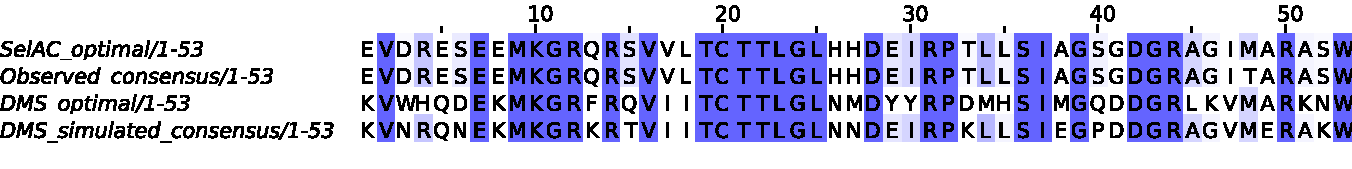
\includegraphics[width=\textwidth]{img/seq_simil_short.pdf}
	\caption{Every 5th residue. DMS and simulation based on DMS do not reflect natural sequences}
	\label{fig:sim_seqs_cons}
\end{figure}

\begin{figure}[h]
    \centering
    \begin{subfigure}
        \centering
        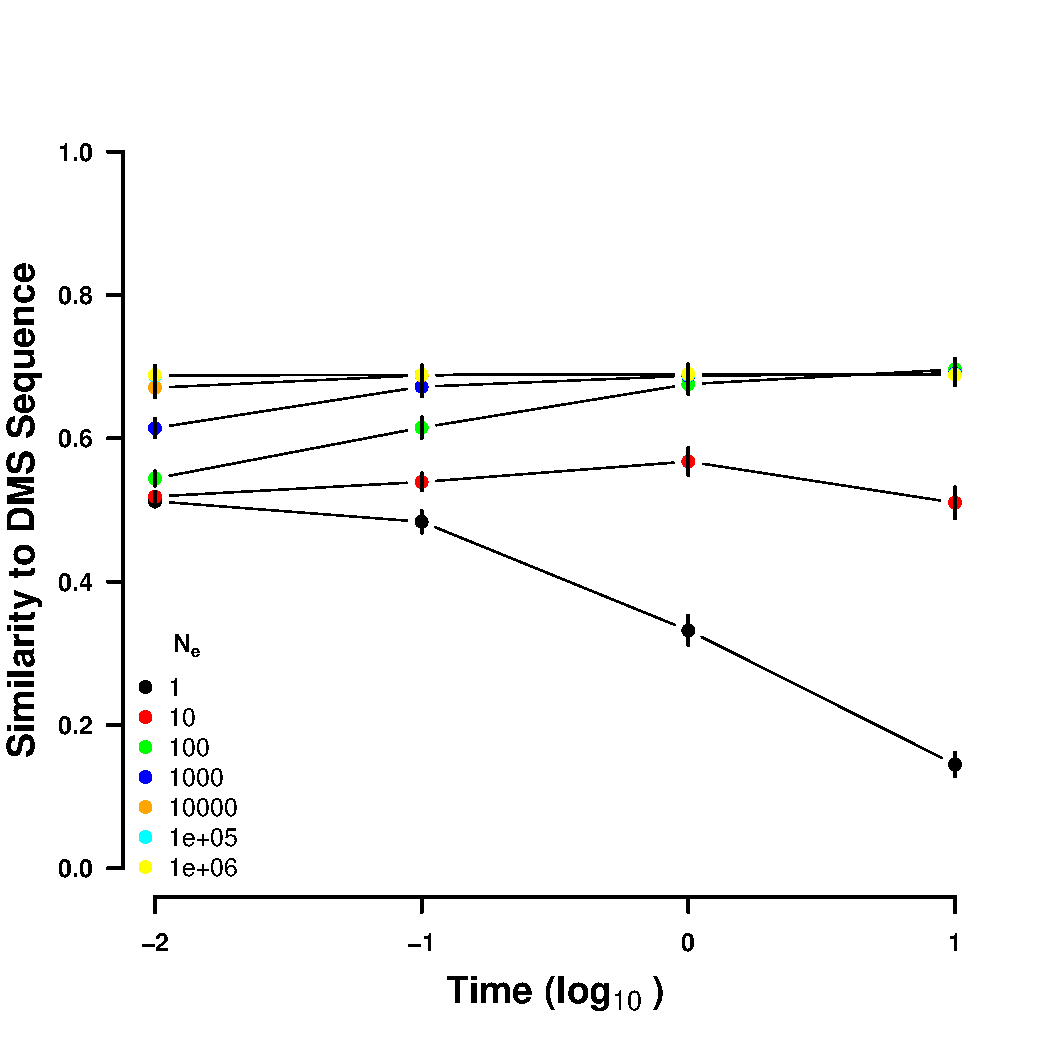
\includegraphics[width=.45\textwidth]{img/simulated_dist_time.pdf}
    \end{subfigure}
    \begin{subfigure}
        \centering
        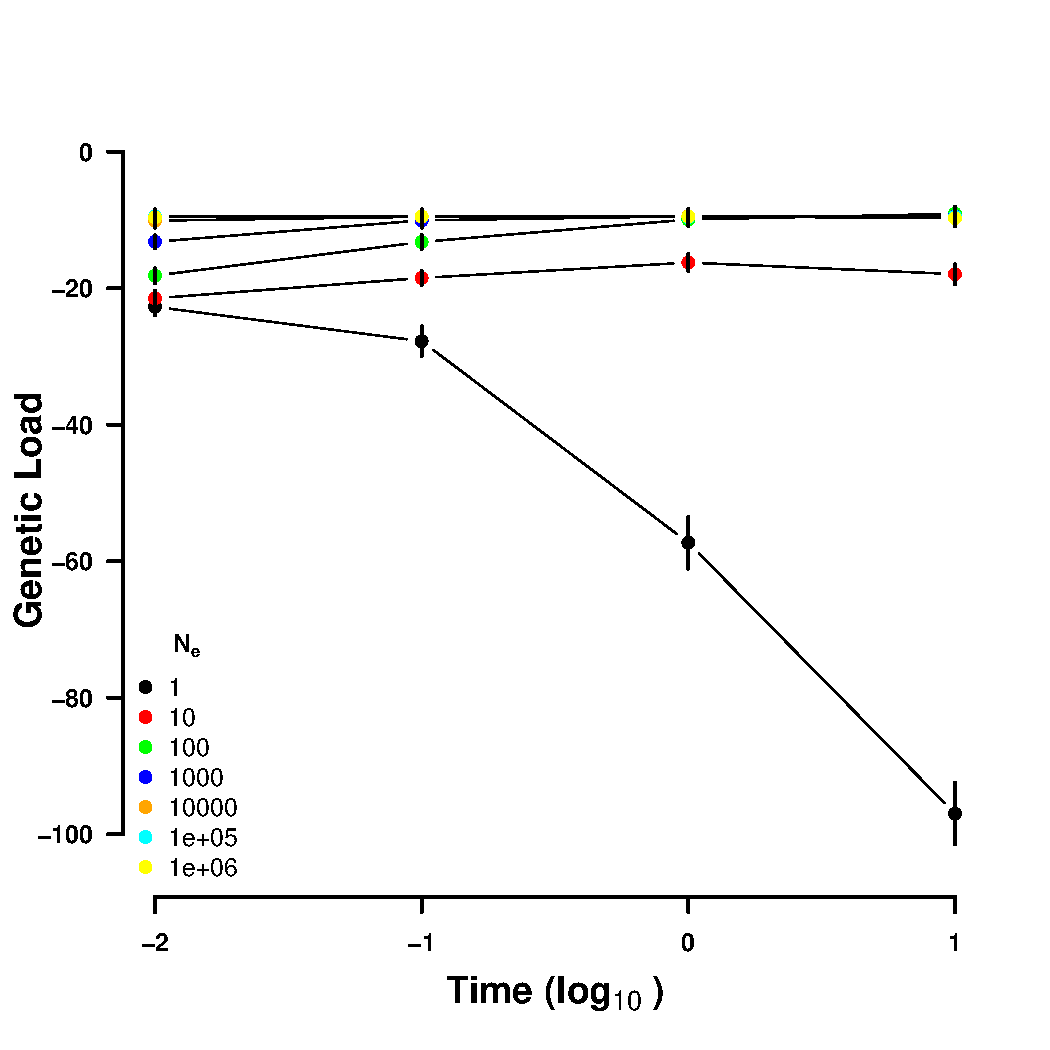
\includegraphics[width=.45\textwidth]{img/simulated_gl_time.pdf}
    \end{subfigure}
    \caption{Sequences simulated under various values of $N_e$ and for various times.}
    \label{fig:dms_sim}
\end{figure}

\begin{figure}[H]
     \centering
	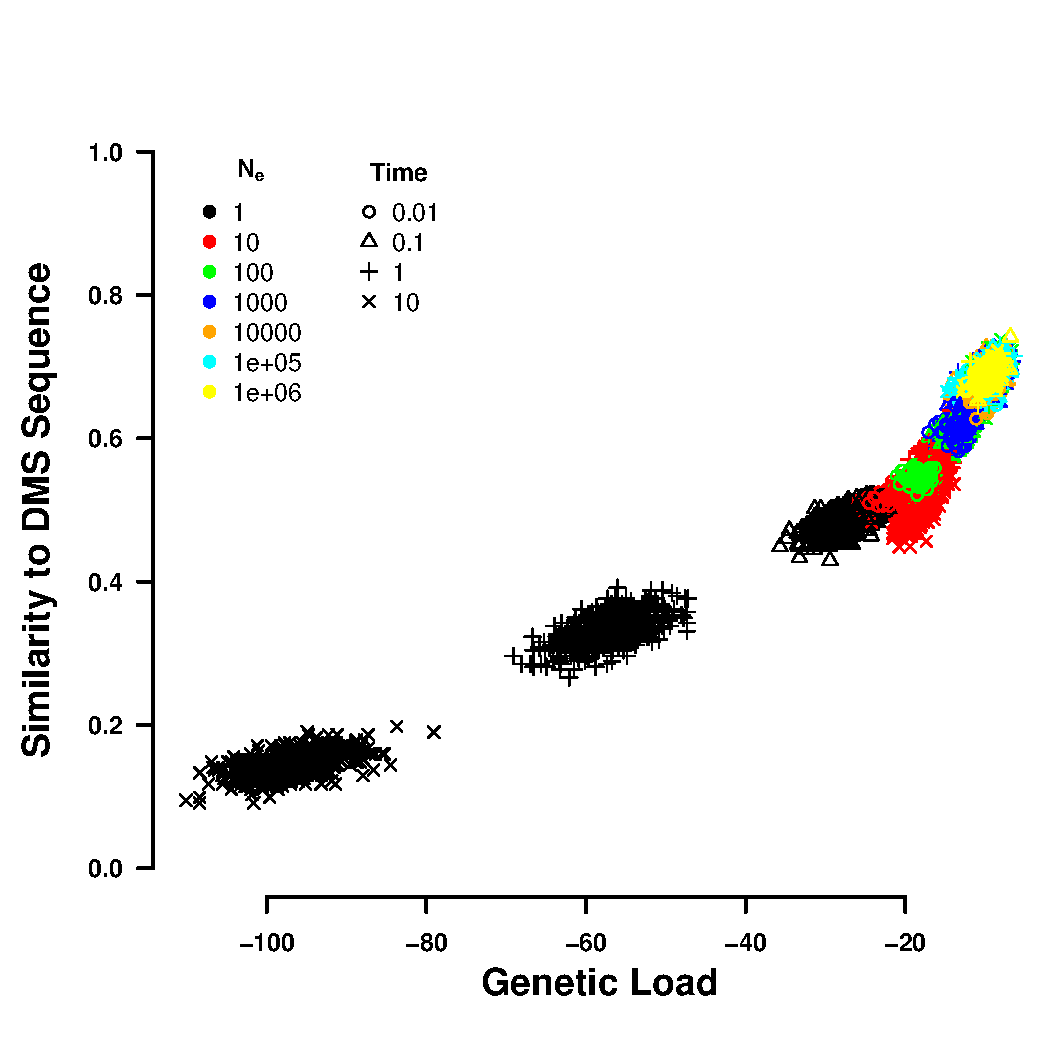
\includegraphics[width=0.6\textwidth]{img/simulated_seqs_gl_dist.pdf}
	\caption{Suppl: Sequences simulated under various values of $N_e$ and for various times. TODO: replace clouds by mean+sd bars}
	\label{fig:sim_seqs}
\end{figure}


\begin{figure}[h]
    \centering
    \begin{subfigure}
        \centering
        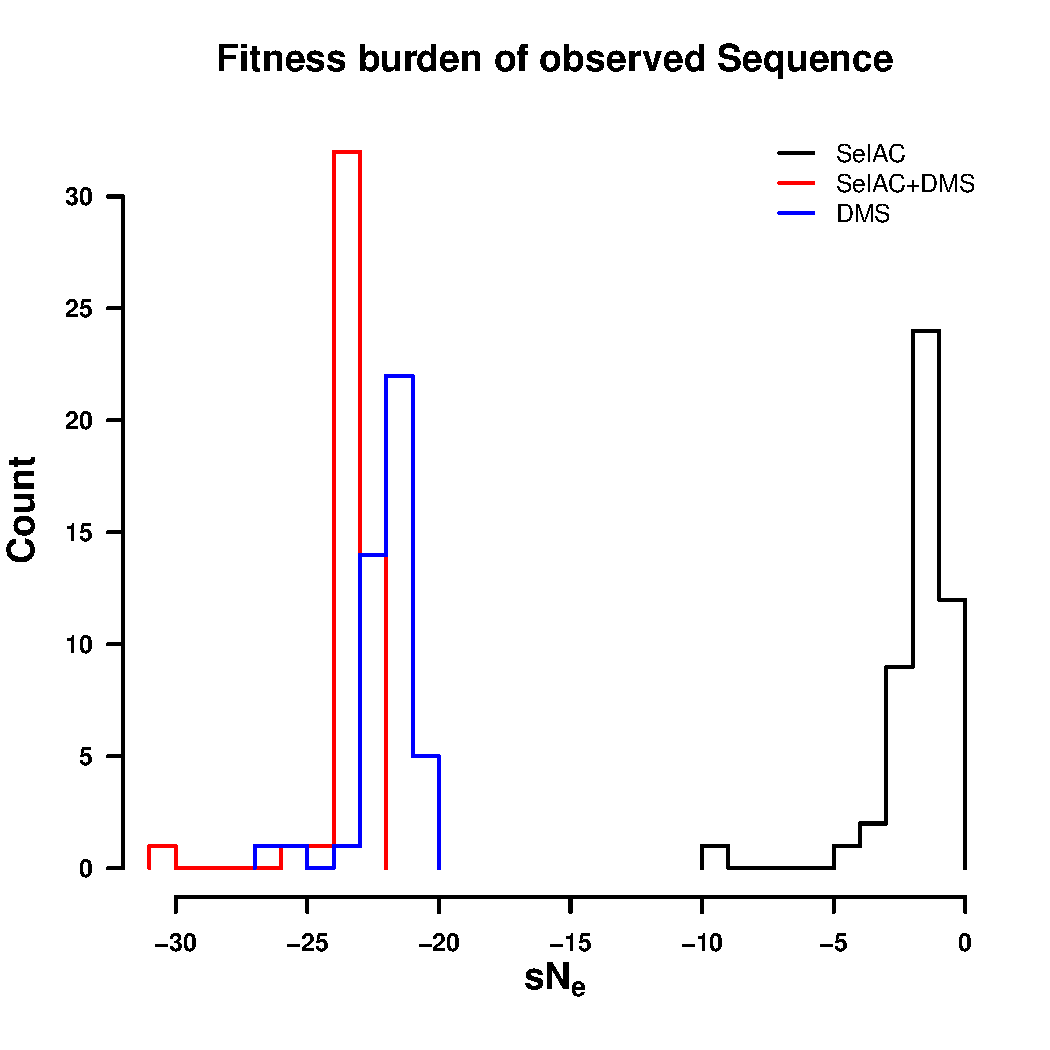
\includegraphics[width=.45\textwidth]{img/sNe_TEM2016.pdf}
    \end{subfigure}
    \begin{subfigure}
        \centering
        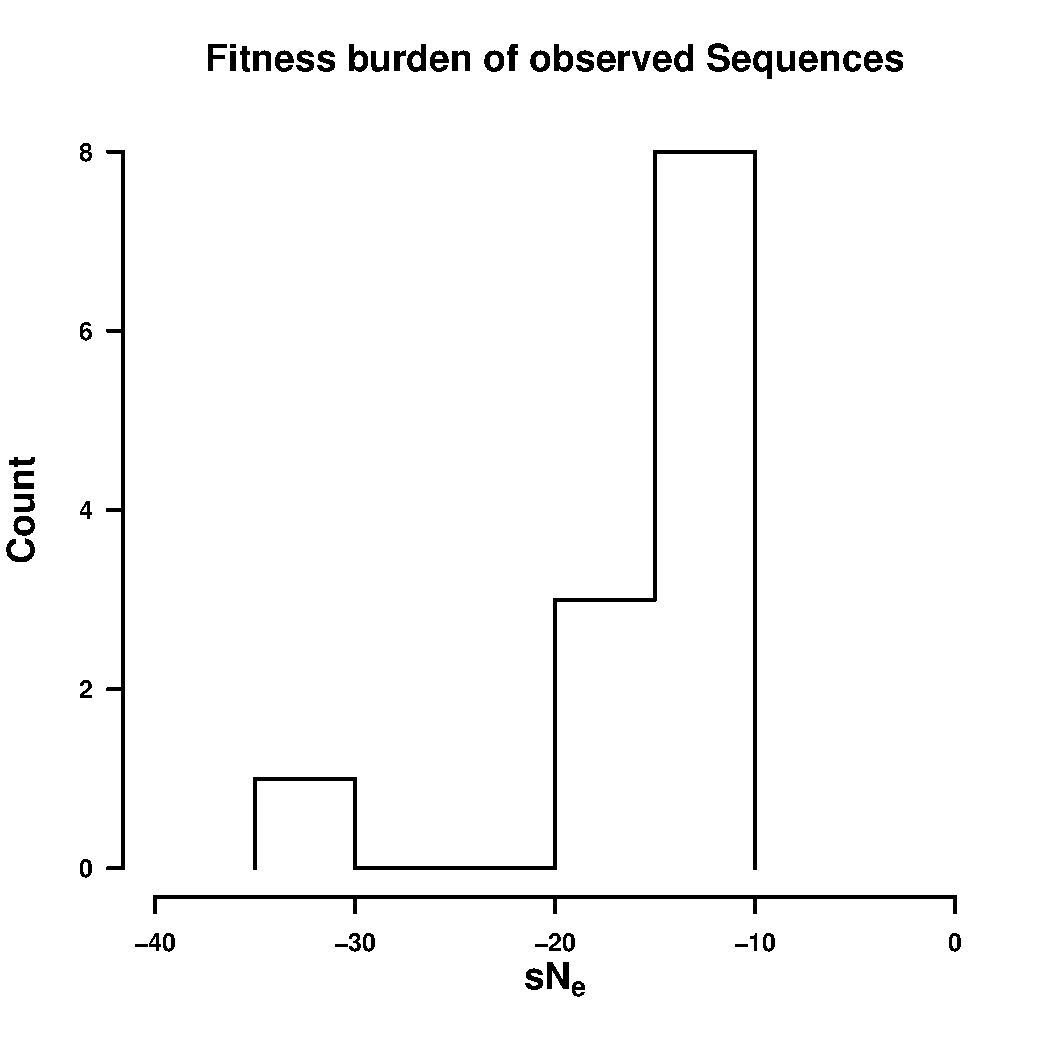
\includegraphics[width=.45\textwidth]{img/sNe_whale.pdf}
    \end{subfigure}
    \caption{$sN_e$ of whole sequence, variation across tips. TEM(left), CytB(right)}
    \label{fig:gl_TEM_whale}
\end{figure}



\begin{figure}[H]
     \centering
	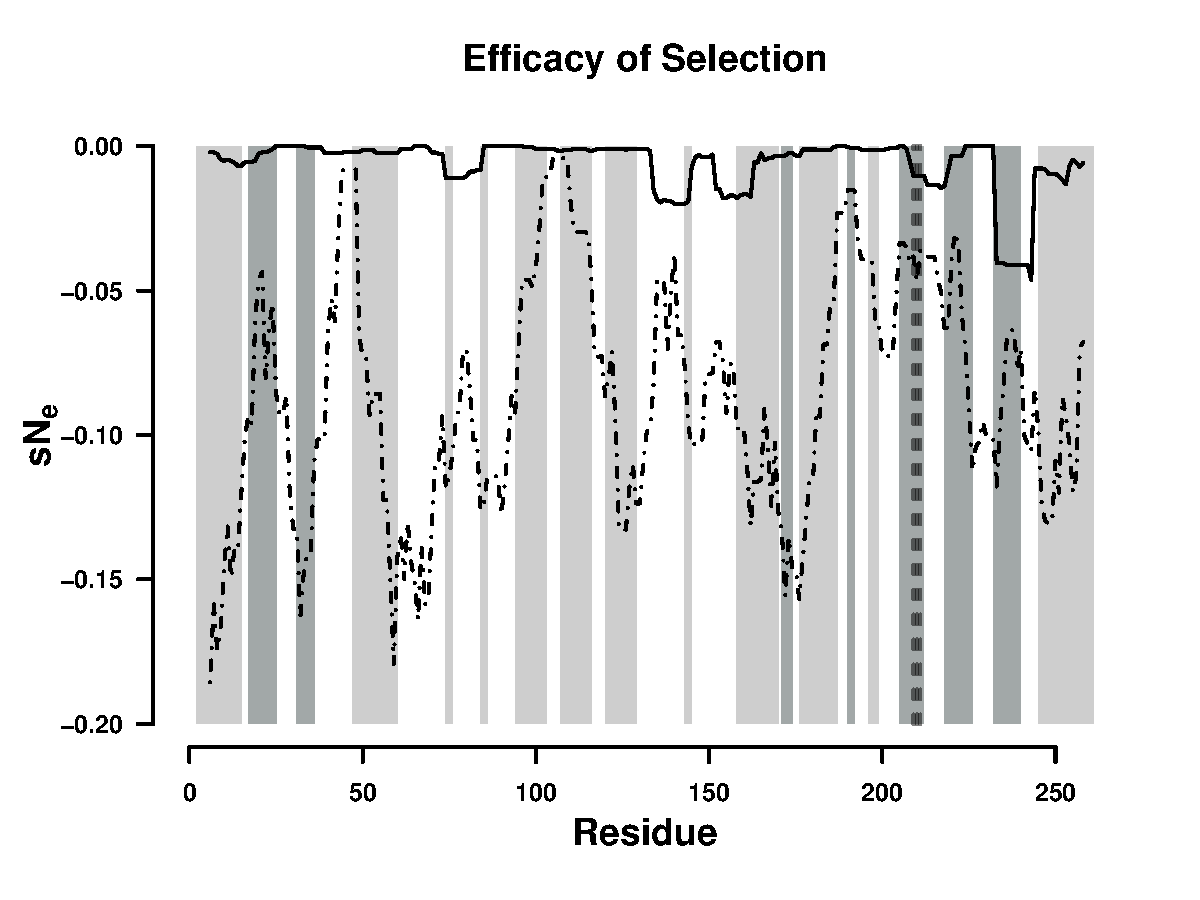
\includegraphics[width=\textwidth]{img/sNe_slide_TEM2016}
	\caption{TEM, bars are different seconday structure elements. Dashed dotted line is DMS, solid is SelAC sNe, all lines are means of all sequences, sliding window of 10 sites. vertical lines are active/binding sites.,}
	\label{fig:tem2016_sse}
\end{figure}

\begin{figure}[H]
     \centering
	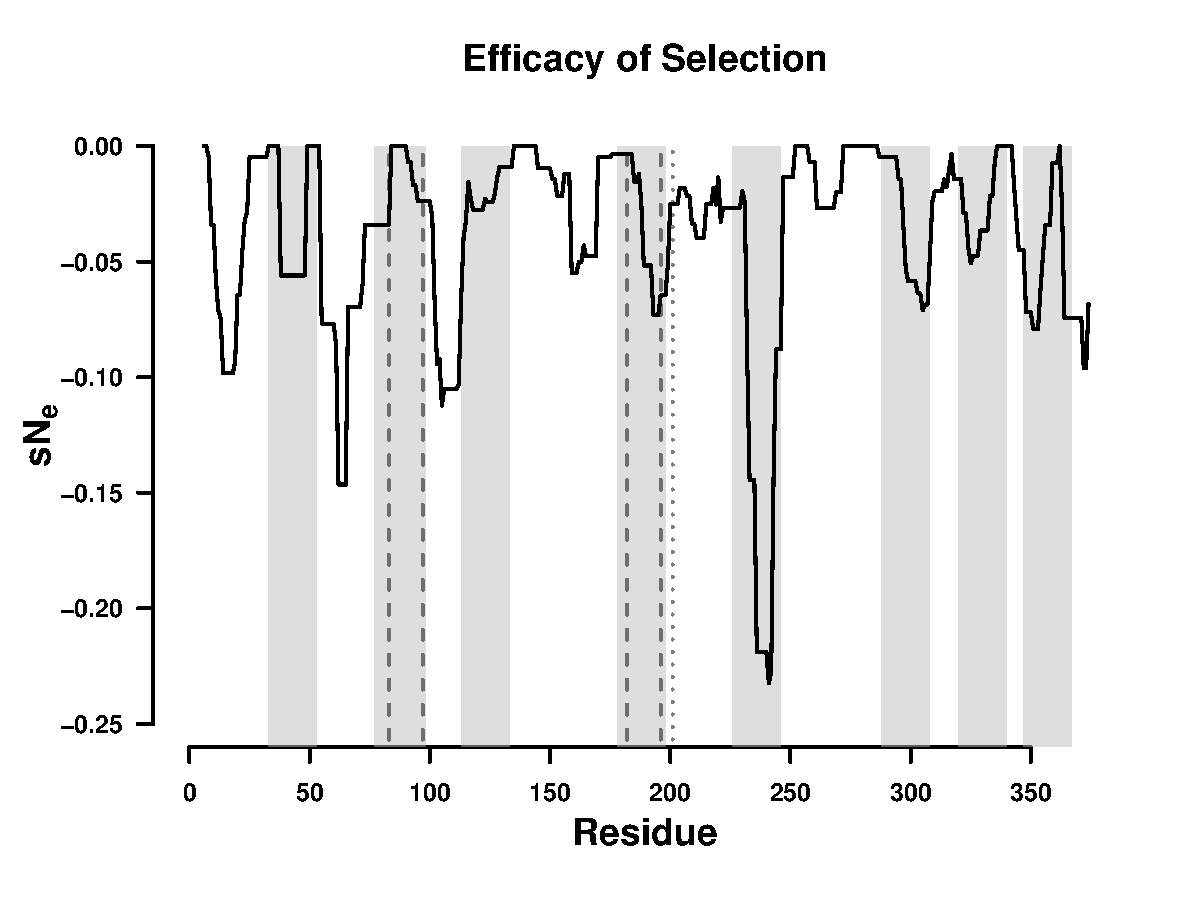
\includegraphics[width=\textwidth]{img/sNe_slide_whale}
	\caption{solid lines is average Genetic Load of CytB alignment,. dashed and dotted lines are different types ofbinding sites. Horizontal bars are alpha helices.}
	\label{fig:whale_sse}
\end{figure}

\end{document}







